% NOTES:
% enum slide
% difference between := and =
% link and plink pic
% filter pic
% examples of running chisel

\documentclass[xcolor=pdflatex,dvipsnames,table]{beamer}
\usepackage{epsfig,graphicx}
\usepackage{palatino}
\usepackage{fancybox}
\usepackage{relsize}
\usepackage[procnames]{listings}

% "define" Scala
\usepackage[T1]{fontenc}  
\usepackage[scaled=0.82]{beramono}  
\usepackage{microtype} 

\sbox0{\small\ttfamily A}
\edef\mybasewidth{\the\wd0 }

\lstdefinelanguage{scala}{
  morekeywords={abstract,case,catch,class,def,%
    do,else,extends,false,final,finally,%
    for,if,implicit,import,match,mixin,%
    new,null,object,override,package,%
    private,protected,requires,return,sealed,%
    super,this,throw,trait,true,try,%
    type,val,var,while,with,yield},
  sensitive=true,
  morecomment=[l]{//},
  morecomment=[n]{/*}{*/},
  morestring=[b]",
  morestring=[b]',
  morestring=[b]"""
}

\usepackage{color}
\definecolor{dkgreen}{rgb}{0,0.6,0}
\definecolor{gray}{rgb}{0.5,0.5,0.5}
\definecolor{mauve}{rgb}{0.58,0,0.82}

% Default settings for code listings
\lstset{frame=tb,
  language=scala,
  aboveskip=3mm,
  belowskip=3mm,
  showstringspaces=false,
  columns=fixed, % basewidth=\mybasewidth,
  basicstyle={\small\ttfamily},
  numbers=none,
  numberstyle=\footnotesize\color{gray},
  % identifierstyle=\color{red},
  keywordstyle=\color{blue},
  commentstyle=\color{dkgreen},
  stringstyle=\color{mauve},
  frame=single,
  breaklines=true,
  breakatwhitespace=true,
  procnamekeys={def, val, var, class, trait, object, extends},
  procnamestyle=\ttfamily\color{red},
  tabsize=2
}

\lstnewenvironment{scala}
{\lstset{language=scala}}
{}
\lstnewenvironment{cpp}
{\lstset{language=C++}}
{}
\lstnewenvironment{bash}
{\lstset{language=bash}}
{}
\lstnewenvironment{verilog}
{\lstset{language=verilog}}
{}


\lstset{basicstyle={\footnotesize\ttfamily}}

\usetheme[height=8mm]{Rochester}
\setbeamersize{text margin left=3mm} 
\setbeamersize{text margin right=3mm} 
\setbeamertemplate{navigation symbols}{}

\definecolor{Cobalt}{rgb}{0.25,0.125,0.70}
\definecolor{RedOrange}{rgb}{0.8,0.25,0.0}
% \definecolor{RedOrange}{rgb}{0.8,0.775,0.25}
\def\frametitledefaultcolor{Cobalt}
\def\frametitleproblemcolor{RedOrange}

\lstset{basicstyle={\footnotesize\ttfamily}}

\setbeamertemplate{frametitle}
{
\vskip-7mm
\textbf{\insertframetitle}\hfill\insertframenumber
}
\setbeamercolor{frametitle}{bg=\frametitledefaultcolor}

\newenvironment{sample}{\VerbatimEnvironment\begin{footnotesize}\begin{semiverbatim}}{\end{semiverbatim}\end{footnotesize}}

\newenvironment{FramedSemiVerb}%
{\begin{Sbox}\begin{minipage}{.94\textwidth}\begin{semiverbatim}}%
{\end{semiverbatim}\end{minipage}\end{Sbox}
\setlength{\fboxsep}{8pt}\fbox{\TheSbox}}

\newenvironment{FramedVerb}%
{\VerbatimEnvironment
\begin{Sbox}\begin{minipage}{.94\textwidth}\begin{Verbatim}}%
{\end{Verbatim}\end{minipage}\end{Sbox}
\setlength{\fboxsep}{8pt}\fbox{\TheSbox}}

% \newenvironment{sample}{\VerbatimEnvironment\begin{footnotesize}\begin{Verbatim}}{\end{Verbatim}\end{footnotesize}}
\newcommand{\code}[1]{\begin{footnotesize}{\tt #1}\end{footnotesize}}
\newcommand{\comment}[1]{{\color{Green}\it\smaller #1}}


\title{Chisel @ CS250 -- Part II -- Lecture 07}
\author{Jonathan Bachrach}
\date{\today}
\institute[UC Berkeley]{EECS UC Berkeley}

\begin{document}

\begin{frame}
\titlepage
\end{frame}
\addtocounter{framenumber}{-1}

% \begin{frame}[fragile]{Forward Declarations using Wires}
% 
% \begin{scala}
% val pcPlus4      = UInt() 
% val branchTarget = UInt()
% val pcNext       = Mux(pcSel, branchTarget, pcPlus4)
% val pcReg        = Reg(data = pcNext, resetVal = UInt(0, 32)) 
% pcPlus4         := pcReg + UInt(4) 
% ... 
% branchTarget    := addOut
% \end{scala}
% 
% \begin{center}
% 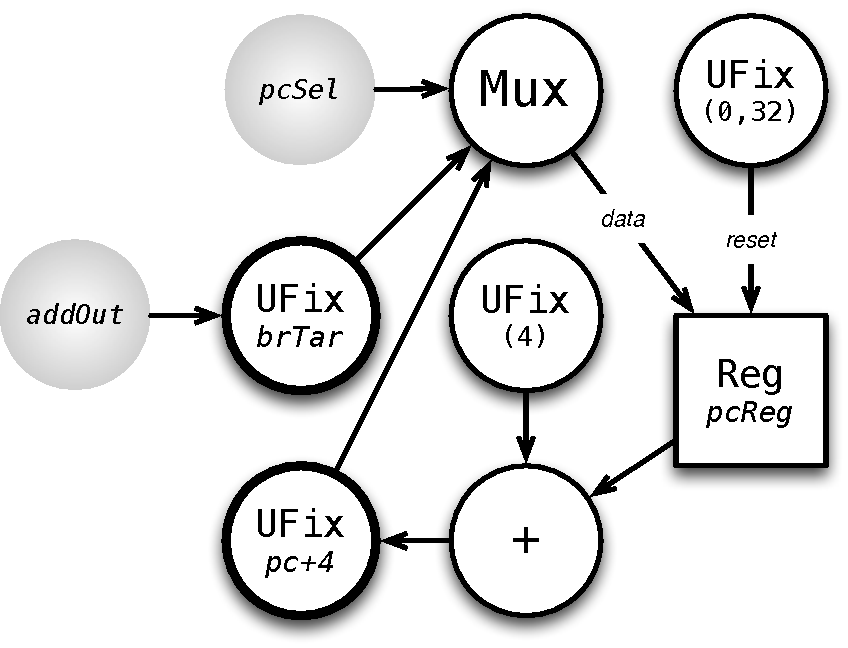
\includegraphics[height=0.5\textheight]{figs/forward.pdf} 
% \end{center}
% 
% \end{frame}

\begin{frame}[fragile]
\frametitle{Accelerator Chisel Interface}
\begin{columns}
\column{0.45\textwidth}
{\lstset{basicstyle={\tiny\ttfamily}}
\begin{scala}
def class MemReq extends Bundle {
  val cmd     = UInt(width = 2)
  val mtype   = UInt(width = 2)
  val tag     = UInt(width = 9)
  val addr    = UInt(width = 64)
  val data    = UInt(width = 64)
}

def class MemResp extends Bundle {
  val cmd     = UInt(width = 2)
  val tag     = UInt(width = 9)
  val mtype   = UInt(width = 2)
  val data    = UInt(width = 64)
}
\end{scala}
\begin{scala}
def class OpReq extends Bundle {
  val code = new RoccInst()
  val a    = UInt(width = 64)
  val b    = UInt(width = 64)
}

def class OpResp extends Bundle {
  val idx  = UInt(width = 5)
  val data = UInt(width = 64)
}
\end{scala}

}

\column{0.45\textwidth}

{\lstset{basicstyle={\tiny\ttfamily}}
\begin{scala}
def class RoccIO extends Bundle {
  val busy    = Bool(OUTPUT)
  val isIntr  = Bool(OUTPUT)
  val memReq  = Decoupled(new MemReq).flip
  val memResp = Decoupled(new MemResp)
  val opReq   = Decoupled(new OpReq)
  val opResp  = Decoupled(new OpResp).flip
}
\end{scala}
}
\begin{center}
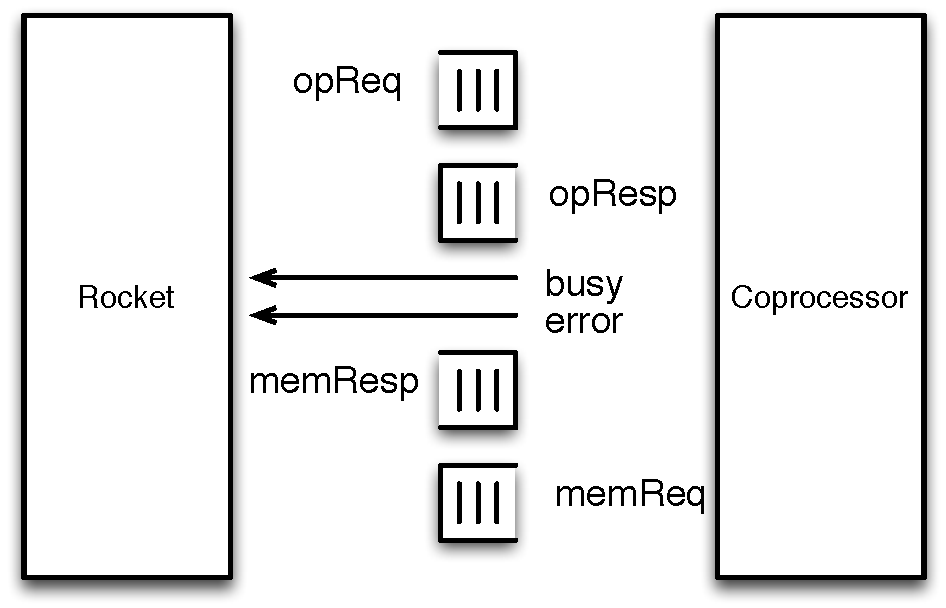
\includegraphics[width=0.9\textwidth]{figs/rocket-coprocessor.pdf}
\end{center}

\end{columns}
\end{frame}

\begin{frame}[fragile]{Accelerator Clarifications}
\begin{columns}
\column{0.45\textwidth}
\begin{itemize}
\item tags on write commands,
\item responses to write commands,
\item must keep busy asserted until all reads and writes have completed, and
\item memory system has single port with accelerator having priority
\end{itemize}
\column{0.45\textwidth}
\begin{center}
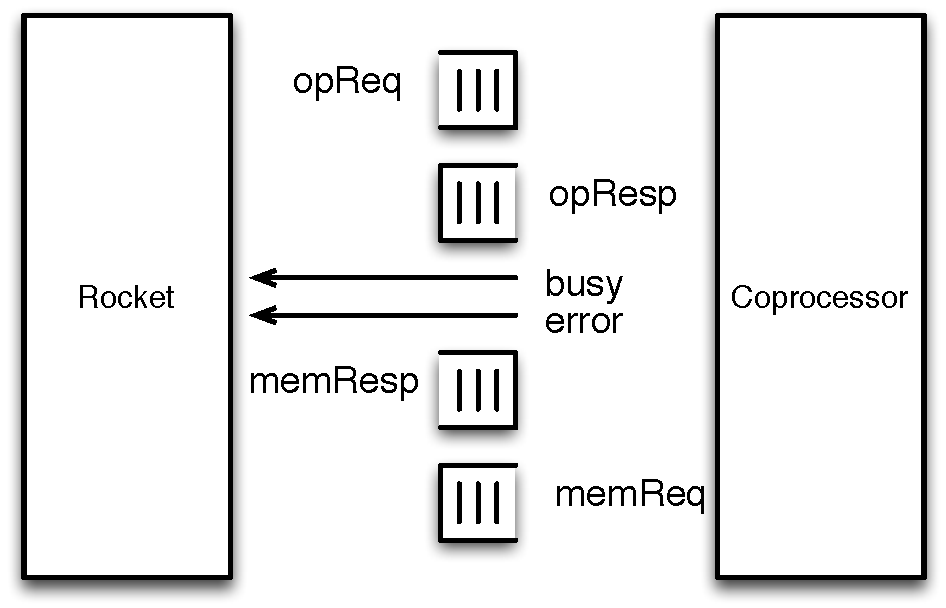
\includegraphics[width=0.9\textwidth]{figs/rocket-coprocessor.pdf}
\end{center}
\end{columns}
\end{frame}

\begin{frame}[fragile]{What is Chisel?}
\begin{itemize}
\item Chisel is just a set of class definitions in Scala and
 when you write a Chisel program you are actually writing a Scala program,
\item Chisel programs produce and manipulate a data structure in Scala using a convenient textural language layered on top of Scala,
\item Chisel makes it possible to create powerful and reusable hardware modules using modern programming language concepts, and
\item the same Chisel description can generate different types of output
\end{itemize}
\end{frame}

\begin{frame}[fragile]{Today}
\begin{itemize}
\item conditional updates on wires, registers, and memories,
\item give you perspective,
\item roms and rams,
\item abstraction through object orientation and functional programming,
\item present how to make hierarchical modules, 
\item teach you how to make reusable modules,
\item show you to even more powerful construction techniques.
\item introduce you to the standard library
\end{itemize}
\end{frame}

\begin{frame}[fragile]{Conditional Updates}
When describing state operations, we could simply wire register inputs to combinational logic blocks, but it is often more convenient:
\begin{itemize}
\item to specify when updates to registers will occur and
\item to specify these updates spread across several separate statements
\end{itemize}

\begin{columns}
\column{0.45\textwidth}
\begin{scala}
val r = Reg( UInt(width = 16) )
when (c === UInt(0) ) {
  r := r + UInt(1)
}
\end{scala}

\column{0.45\textwidth}

\begin{center}
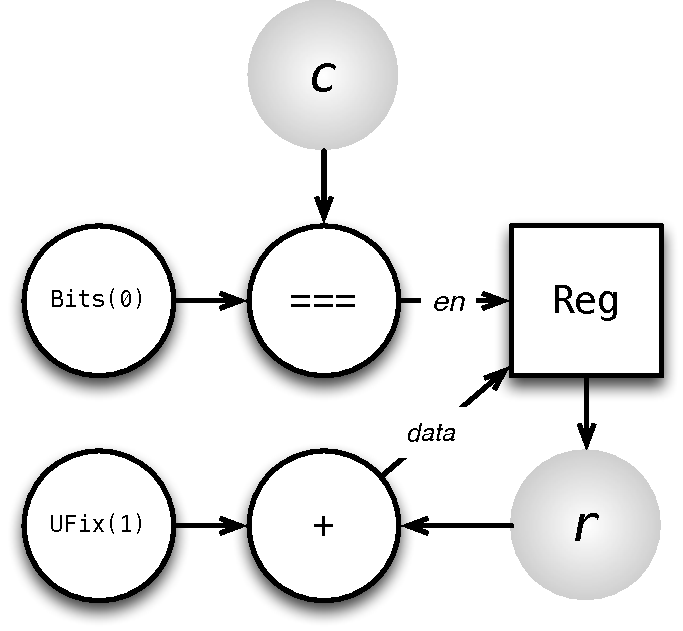
\includegraphics[width=0.9\textwidth]{figs/conditional-increment.pdf} 
\end{center}

\end{columns}
\end{frame}

\begin{frame}[fragile]{Conditional Updates Priority}

\begin{scala}
when (c1) { r := Bits(1) }
when (c2) { r := Bits(2) }
\end{scala}

\textbf{Conditional Update Order:}

\begin{center}
\begin{tabular}{|c|c|c|l|}
\hline
\code{c1} & \code{c2}  &  \code{r} & \\
\hline
0 &  0 & r &  \code{r} unchanged \\
0 &  1 & 2 & \\
1 &  0 & 1 & \\
1 &  1 & 2 & \code{c2} takes precedence over \code{c1} \\
\hline
\end{tabular}
\end{center}

\end{frame}

\begin{frame}[fragile]{Conditional Update Synthesized Hardware}

\begin{center}
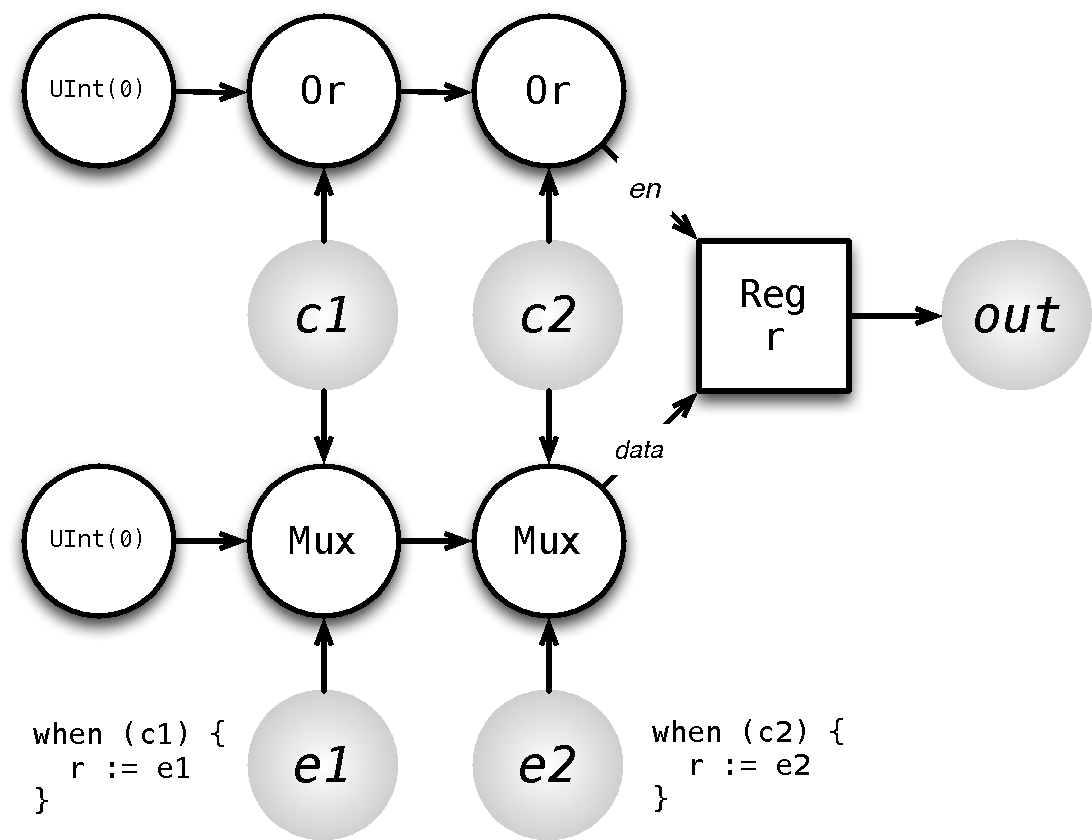
\includegraphics[height=2in]{figs/conditional-updates.pdf}
\end{center}

\begin{itemize}
\item Each \code{when} statement adds another level of data mux and ORs
  the predicate into the enable chain and
\item the compiler effectively adds
  the termination values to the end of the chain automatically.
\end{itemize}

\end{frame}

\begin{frame}[fragile]{Targetting Multiple Registers}

\begin{scala}
r := Reg( init = UInt(3) )
s := Reg( init = UInt(3) )
when (c1) { r := UInt(1); s := UInt(1) }
when (c2) { r := UInt(2) }
\end{scala}

leads to \code{r} and \code{s} being updated according to the
following truth table:

{\footnotesize
\begin{center}
\begin{tabular}{|c|c|c|c|l|}
\hline
\code{c1} & \code{c2}  & \code{r} & \code{s} & \\
\hline 
0 &  0 & 3 & 3 & \\
0 &  1 & 2 & 3 & \\ 
1 &  0 & 1 & 1 & \code{r} updated in \code{c2} block, \code{s} updated using default \\
1 &  1 & 2 & 1 & \\
\hline
\end{tabular}
\end{center}
}

\end{frame}

\begin{frame}[fragile]{Conditional Update Nesting}

\begin{scala}
when (a) { when (b) { body } }
\end{scala}

which is the same as:

\begin{scala}
when (a && b) { body }
\end{scala}

\end{frame}

\begin{frame}[fragile]{Conditional Update Chaining}

\begin{scala}
when (c1) { u1 }
.elsewhen (c2) { u2 }
.otherwise { ud }
\end{scala}

which is the same as:

\begin{scala}
when (c1) { u1 }
when (!c1 && c2) { u2 }
when (!(c1 || c2)) { ud }
\end{scala}

\end{frame}

\begin{frame}[fragile]{Switch Statement}

\begin{scala}
switch(idx) {
  is(v1) { u1 }
  is(v2) { u2 }
}
\end{scala}

which is the same as:

\begin{scala}
when (idx === v1) { u1 }
when (idx === v2) { u2 }
\end{scala}

\end{frame}

% \begin{frame}[fragile]{Enums}
% \begin{scala}
% val s_even :: s_odd :: Nil = Enum(2){ UInt() }
% \end{scala}
% \end{frame}


\begin{frame}[fragile]{Conditional Updates Everywhere}
Conditional updates also work for 
\begin{itemize}
\item wires but must have defaults and
\item for memory reads and writes as we'll see soon...
\end{itemize}

For wires, we can do conditional updates as follows:

\begin{scala}
val w = Bits(width = 32)
w := Bits(0)                       // default value 
when (c1)         { w := Bits(1) }
when (c2)         { w := Bits(2) }
\end{scala}

\noindent
which is the same as

\begin{scala}
val w = Bits(width = 32)
when (Bool(true)) { w := Bits(0) } // default value
when (c1)         { w := Bits(1) }
when (c2)         { w := Bits(2) }
\end{scala}

\end{frame}

\begin{frame}[fragile]{Enums}
Enums can be defined to create a list of increasing nums.

\begin{scala}
object Enum {
  def apply[T <: UInt](type: T, n: Int): List[T] = ...
}
\end{scala}

\begin{scala}
val s_even :: s_odd :: Nil = Enum(UInt(), 2)
\end{scala}

\end{frame}

\begin{frame}[fragile]{Finite State Machines}

\begin{columns}
\column{0.65\textwidth}

Finite state machines can now be readily defined as follows:

\begin{scala}
class Parity extends Module {
  val io = new Bundle {
    val in  = Bool(INPUT)
    val out = Bool(OUTPUT) }
  val s_even :: s_odd :: Nil = Enum(UInt(), 2)
  val state  = Reg(resetVal = s_even)
  when (io.in) {
    when (state === s_even) { state := s_odd  }
    .otherwise              { state := s_even }
  }
  io.out := (state === s_odd)
}
\end{scala}

\column{0.25\textwidth}

\begin{center}
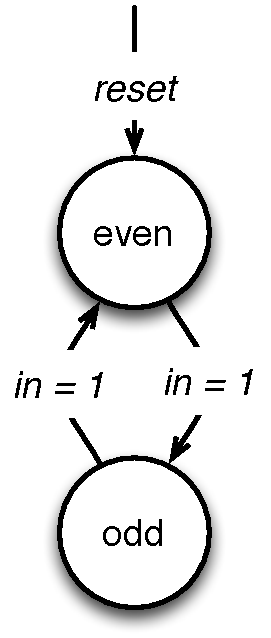
\includegraphics[height=0.9\textheight]{figs/parity.pdf} 
\end{center}

\end{columns}
\end{frame}

\input{../talks/microsoft/libs-to-langs-guts.tex}


\begin{frame}[fragile]{ROM}

\begin{scala}
val d = Array(UInt(1), UInt(2), UInt(4), UInt(8))
val m = ROM(UInt(width = 32), d)
val r = m(counter(UInt(3)))
\end{scala}

\begin{center}
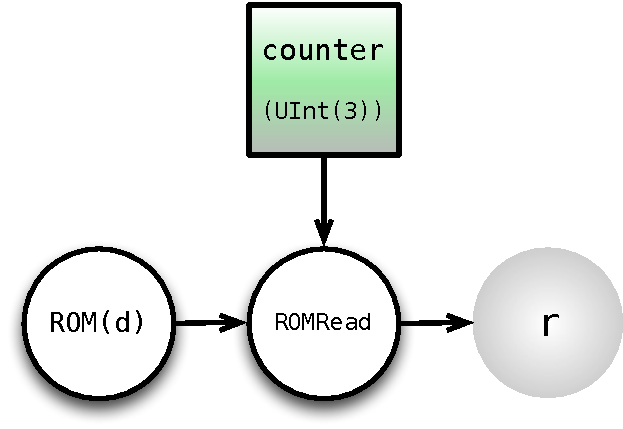
\includegraphics[height=0.7\textheight]{figs/rom.pdf} 
\end{center}

\end{frame}

\begin{frame}[fragile]{Mul Lookup Table}
\begin{columns}
\column{0.52\textwidth}

\begin{scala}
class Mul extends Module {
  val io = new Bundle {
    val x   = UInt(INPUT, 4)
    val y   = UInt(INPUT, 4)
    val z   = UInt(OUTPUT, 8) }

  val muls = new Array[UInt](256)
  for (x <- 0 until 16; y <- 0 until 16) 
    muls((x << 4) | y) = UInt(x * y)

  val tbl = ROM(UInt(8), muls)

  io.z := tbl((io.x << 4) | io.y)
}
\end{scala}

\column{0.38\textwidth}

\begin{center}
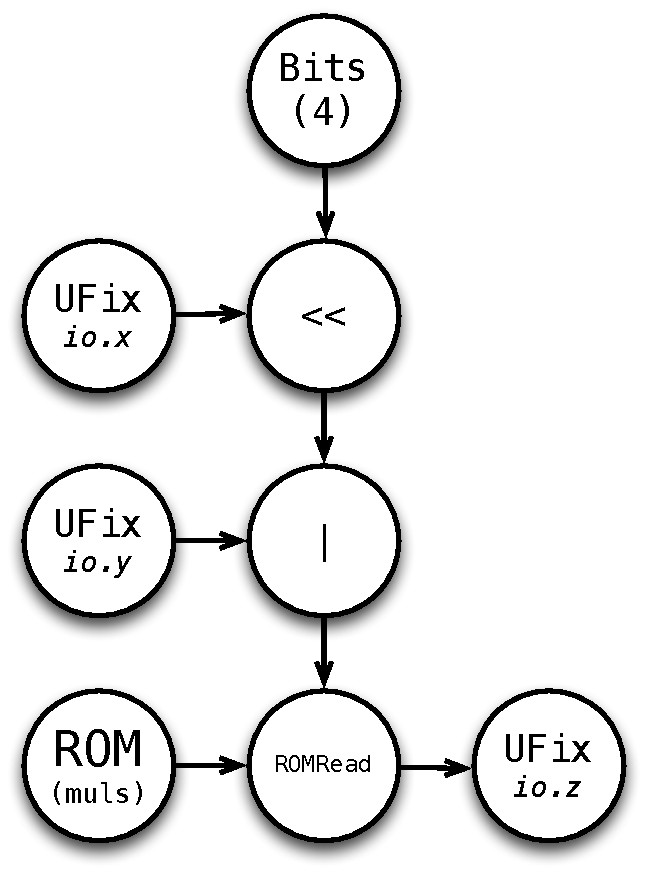
\includegraphics[width=0.9\textwidth]{figs/muls.pdf} 
\end{center}

\end{columns}
\end{frame}

\begin{frame}[fragile]{RAM}
RAM is supported using the \code{Mem} construct

\begin{scala}
val m = Mem(Bits(width = 32), 32)
\end{scala}

\noindent
where
\begin{itemize}
\item writes to Mems are positive-edge-triggered
\item reads are either combinational or positive-edge-triggered
\item ports are created by applying a \code{UInt} index
\end{itemize}
\end{frame}

\begin{frame}[fragile]{32-entry Register File}

\begin{scala}
val regs = Mem(Bits(width = 32), 32)
when (wrEn) {
  regs(wrAddr) := wrData
}
val iDat = regs(iAddr)
val mDat = regs(mAddr)
\end{scala}

\begin{center}
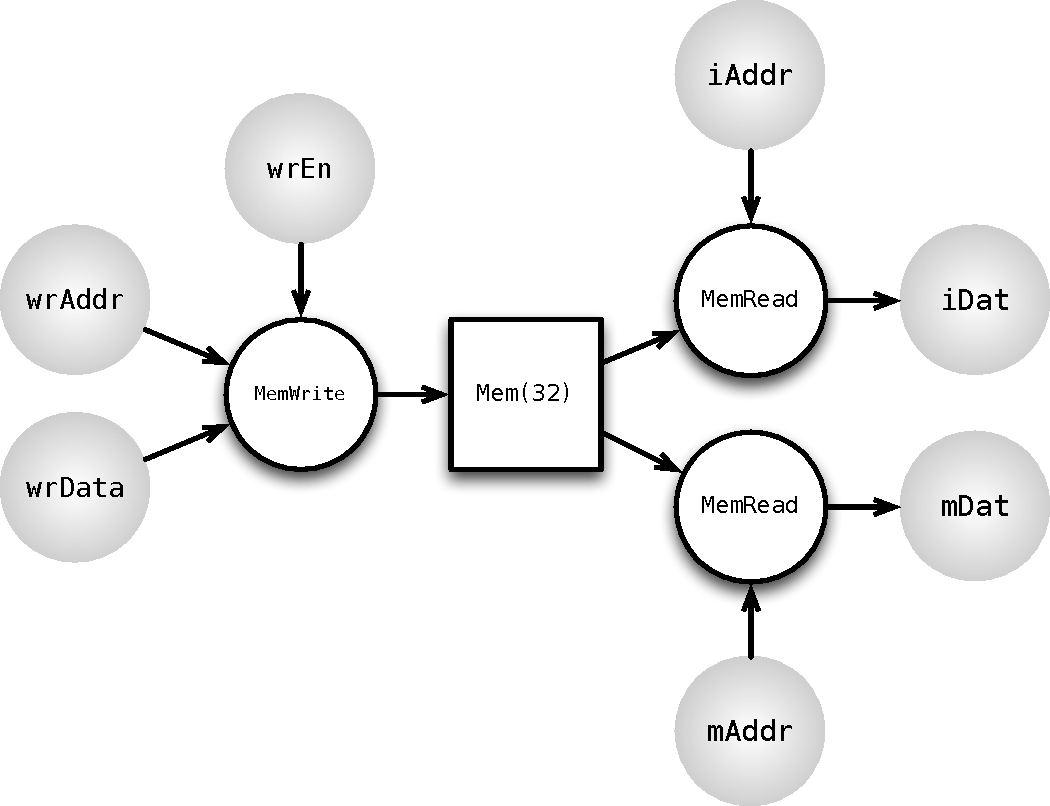
\includegraphics[height=0.55\textheight]{figs/mem.pdf} 
\end{center}

\end{frame}

\begin{frame}[fragile]{Sequential Read Ports}
Sequential read ports are inferred when:
\begin{itemize}
\item optional parameter \code{seqRead} is set and
\item read address is a reg
\end{itemize}

\begin{scala}
al ram1r1w =
  Mem(UInt(width = 32), 1024, seqRead = true)
val reg_raddr = Reg(UInt())
when (wen) { ram1r1w(waddr) := wdata }
when (ren) { reg_raddr := raddr }
val rdata = ram1r1w(reg_raddr)
\end{scala}

\begin{center}
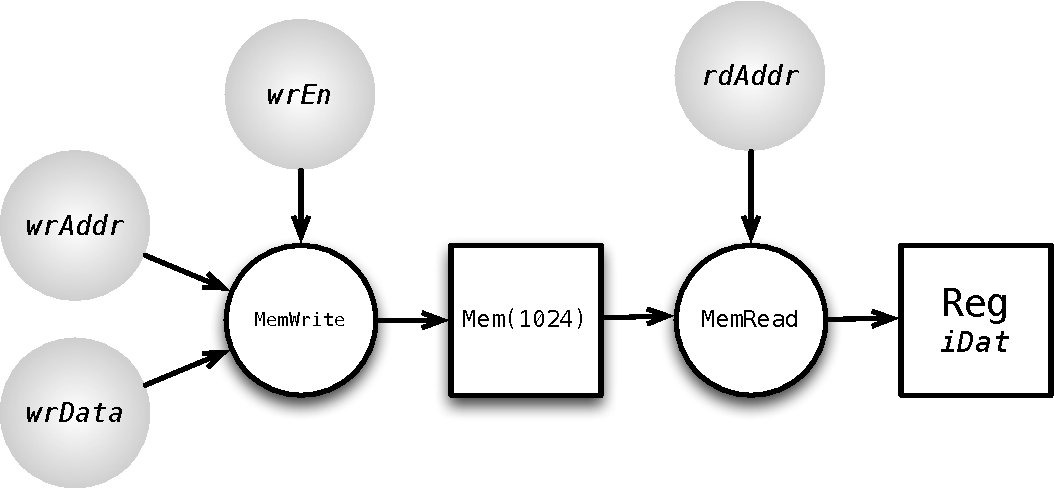
\includegraphics[height=0.4\textheight]{figs/mem-seq-read.pdf} 
\end{center}

\end{frame}

\begin{frame}[fragile]{Single-ported SRAM}
Single-ported SRAMs can be inferred when the read and write conditions are
mutually exclusive in the same \code{when} chain

\begin{scala}
al ram1p =
  Mem(UInt(width = 32), 1024, seqRead = true)
val reg_raddr = Reg(UInt())
when (wen) { ram1p(waddr) := wdata }
.elsewhen (ren) { reg_raddr := raddr }
val rdata = ram1p(reg_raddr)
\end{scala}

\begin{center}
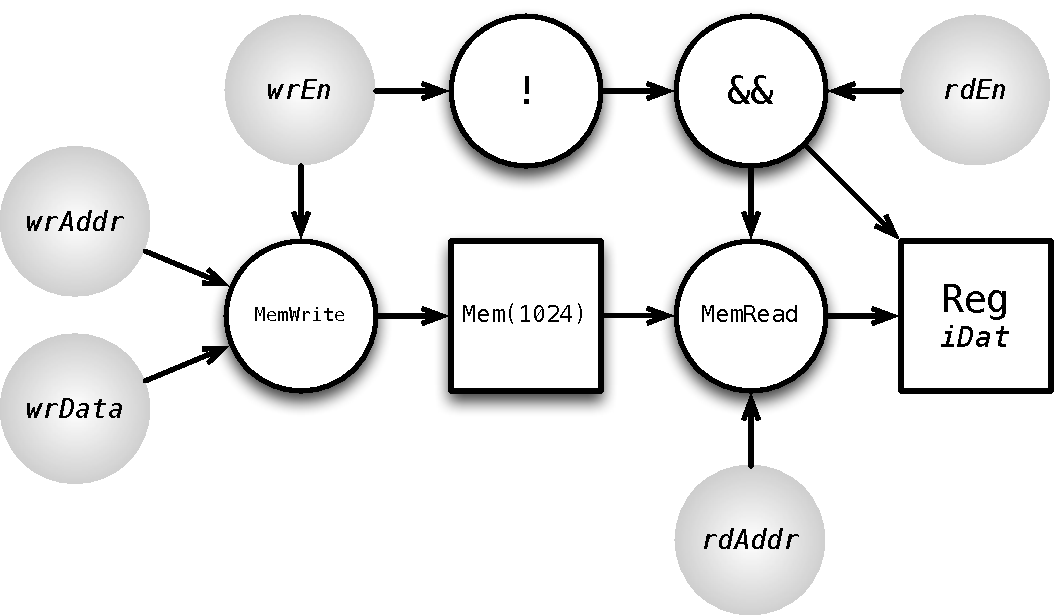
\includegraphics[height=0.5\textheight]{figs/mem-single-ported.pdf} 
\end{center}

\end{frame}

\begin{frame}[fragile]{Mem Write Masks }
Mem also supports write masks for subword writes. 
\begin{itemize}
\item A given bit is written if the corresponding mask bit is set.
\end{itemize}

\begin{scala}
val ram = Mem(UInt(width = 32), 256)
when (wen) { ram.write(waddr, wdata, wmask) }
\end{scala}

\end{frame}

\begin{frame}{Prepare for Warp Speed and Be Happy}
Congratulations, you have all that you need at this point to write Chisel programs!
You can write RTL, define modules (even with recursive data types), and wire them together.
\vspace{5mm}
\begin{itemize}
\item In order to attain true hardware description power though, you need to be able to write reusable RTL, modules and interfaces.
\item This will allow you to both use and write generic module libraries and more quickly explore design space.
\item To do this, we will use modern programming techniques such as:
\begin{itemize}
\item object orientation, 
\item functional programming, 
\item parameterized types
\end{itemize}
\item You will be greatly rewarded for your efforts!
\end{itemize}

\end{frame}

\begin{frame}[fragile]{Parameterized Types in Scala}
First we need to learn about parameterized types in Scala.
We can define a generic \code{Mux} function as taking a boolean condition and \code{con} and \code{alt} arguments (corresponding to then and else expressions) of type \code{T} as follows:

\begin{scala}
def Mux[T <: Data](c: Bool, con: T, alt: T): T = ...
\end{scala}

\noindent
where 
\begin{itemize}
\item \code{T} is required to be a subclass of \code{Data} and 
\item the type of \code{con} and \code{alt} are required to match.
\end{itemize}

\noindent
You can think of the type parameter as a way of just constraining the types of the allowable arguments.

\end{frame}

\begin{frame}[fragile]
\frametitle{Revisiting GCD}
\begin{columns}

\column{0.45\textwidth}

\begin{footnotesize}
\begin{scala}
class GCD extends Module {
  val io = new Bundle {
    val a     = UInt(INPUT, 16)
    val b     = UInt(INPUT, 16)
    val z     = UInt(OUTPUT, 16)
    val valid = Bool(OUTPUT) }
  val x = Reg(init = io.a)
  val y = Reg(init = io.b)
  when (x > y) {
    x := x - y
  } .otherwise {
    y := y - x
  }
  io.z     := x
  io.valid := y === UInt(0)
}
\end{scala}
\end{footnotesize}

\column{0.45\textwidth}

\begin{center}
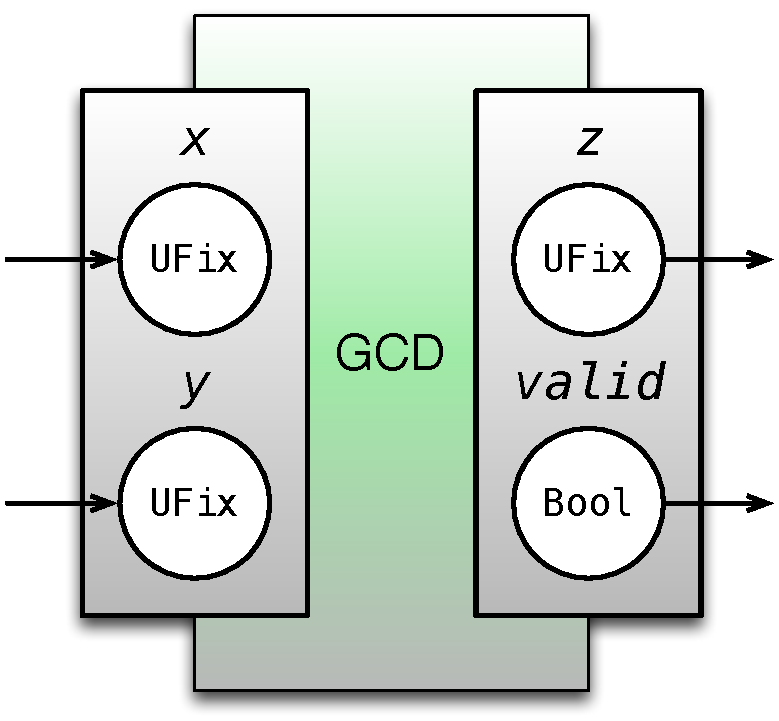
\includegraphics[width=0.9\textwidth]{../talks/retreat-1/figs/gcd.pdf} 
\end{center}

\end{columns}
\note{defining modules is a matter of \\[1cm]
defining its interface and then \\[1cm]
wiring outputs to compute logic and state defined in terms of inputs. \\[1cm]
here we're defining registers and conditional updates on them. \\[1cm]
this module outputs valid true when an answer is ready.}
\end{frame}

\begin{frame}[fragile]
\frametitle{Valid Wrapper}

\begin{columns}

\column{0.65\textwidth}

\begin{footnotesize}
\begin{scala}
class Valid[T <: Data](dtype: T) extends Bundle {
  val data  = dtype.clone
  val valid = Bool()
  override def clone = new Valid(dtype)
}

class GCD extends Module {
  val io = new Bundle {
    val a   = UInt(INPUT, 16)
    val b   = UInt(INPUT, 16)
    val out = new Valid(UInt(OUTPUT, 16))
  } }
  ...
  io.out.data  := x
  io.out.valid := y === UInt(0)
}

\end{scala}
\end{footnotesize}

\column{0.3\textwidth}

\begin{center}
\includegraphics[width=0.9\textwidth]{../talks/retreat-1/figs/valid.pdf} 
\end{center}

\end{columns}
\note{now gcd had a valid signal on its output.  \\[1cm]
we can generalize this idea by defining a wrapper class that bundles a valid with a data signal. \\[1cm]
now we can rewrite GCD using an interface using this valid wrapper for its output. }

\end{frame}

\begin{frame}[fragile]
\frametitle{Function Filters}

\begin{footnotesize}
\begin{scala}
abstract class Filter[T <: Data](dtype: T) extends Module {
  val io = new Bundle {
    val in  = new Valid(dtype).asInput
    val out = new Valid(dtype).asOutput
} }

class FunctionFilter[T <: Data](f: T => T, dtype: T) extends Filter(dtype) {
  io.out.valid := io.in.valid
  io.out       := f(io.in)
}
\end{scala}
\end{footnotesize}

\begin{center}
\includegraphics[height=0.4\textheight]{../talks/sketching13/figs/function-filter.pdf} 
\end{center}

\note{suppose we want to write hardware filters. \\[1cm]
one way to create a reusable filter would be \\[1cm]
to create a filter class that takes a function as argument that definines its filter operation.}

\end{frame}

\begin{frame}[fragile]
\frametitle{Clipping Filter}

\begin{footnotesize}
\begin{scala}
def clippingFilter[T <: Num](limit: Int, dtype: T) = 
  new FunctionFilter(min(limit, max(-limit, _)), dtype)
\end{scala}
\end{footnotesize}

\begin{center}
\includegraphics[height=0.4\textheight]{../talks/retreat-1/figs/clipping-filter.pdf} 
\end{center}
\note{using this reusable substrate then it is easy to create an instance of a filter.}
\end{frame}


\begin{frame}[fragile]
\frametitle{Shifting Filter}

\begin{footnotesize}
\begin{scala}
def shiftingFilter[T <: Num](shift: Int, dtype: T) = 
  new FunctionFilter(_ >> shift, dtype)
\end{scala}
\end{footnotesize}

\begin{center}
\includegraphics[height=0.4\textheight]{../talks/retreat-1/figs/shifting-filter.pdf} 
\end{center}
\note{and reuse it for shift filter}
\end{frame}

\begin{frame}[fragile]
\frametitle{Chained Filter}

\begin{footnotesize}
\begin{scala}
class ChainedFilter[T <: Num](dtype: T) extends Filter(dtype) = {
  val shift   = new ShiftFilter(2, dtype)
  val clipper = new ClippingFilter(1 << 7, dtype)
  io.in          <> shift.io.in
  shift.io.out   <> clipper.io.in
  clipper.io.out <> io.out
}
\end{scala}
% \begin{scala}
% class ChainedFilter[T <: Num](dtype: T) extends Filter(dtype) = {
%   val fir     = new TstFIR(dtype)
%   val shift   = new ShiftFilter(2, dtype)
%   val clipper = new ClippingFilter(1 << 7, dtype)
%   io.in          <> fir.io.in
%   fir.io.out     <> shift.io.in
%   shift.io.out   <> clipper.io.in
%   clipper.io.out <> io.out
% }
% \end{scala}
\end{footnotesize}

\begin{center}
\includegraphics[height=0.4\textheight]{../talks/sketching13/figs/chained-filter2.pdf} 
\end{center}
\note{and chain together...}
\end{frame}

\begin{frame}[fragile, shrink]
\frametitle{Functional Composition}

% \begin{itemize}
% \item natural
% \item reusable
% \item composable
% \end{itemize}
% \vskip1cm

\begin{Large}
\begin{columns}

\column{0.45\textwidth}
\verb+Map(ins, x => x * y)+ \\
\begin{center}
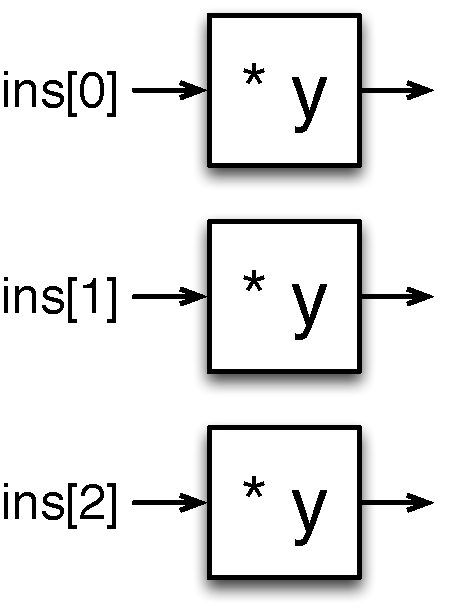
\includegraphics[height=0.6\textheight]{../bootcamp/figs/map.pdf} \\[2cm]
\end{center}

\column{0.45\textwidth}
\vskip2mm
\verb+Chain(n, in, x => f(x))+ \\
\begin{center}
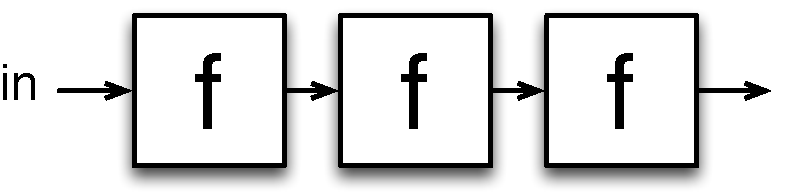
\includegraphics[width=0.9\textwidth]{../bootcamp/figs/chain.pdf} \\
\end{center}

\verb+Reduce(ins, Max)+ \\
\begin{center}
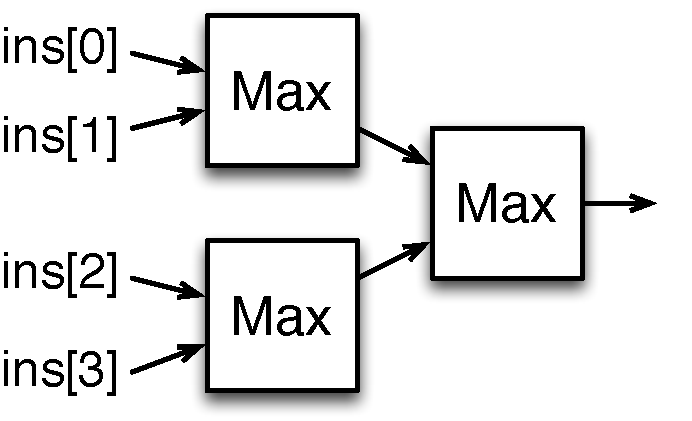
\includegraphics[width=0.9\textwidth]{../bootcamp/figs/reduce.pdf} \\
\end{center}

\end{columns}

\end{Large}
\note{the previous example showed a simple use of functional programming. \\[1cm]
Scala provides strong support for functional programming and
it turns out that functional programming is a powerful way to define hardware. \\[1cm]
for example, you can create a parallel set of blocks using map and reduce to creation reduction trees and chain to create a pipeline.}
\end{frame}

\begin{frame}[fragile]{Generator}
\begin{footnotesize}
\begin{scala}
def delays[T <: Data](x: T, n: Int): List[T] = 
  if (n <= 1) List(x) else x :: taps(Reg(next = x), n-1)

def FIR[T <: Num](hs: Seq[T], x: T): T = 
  (hs, delays(x, hs.length)).zipped.map( _ * _ ).reduce( _ + _ )

class TstFIR extends Module {
  val io = new Bundle{ val x  = SInt(INPUT, 8); val y = SInt(OUTPUT, 8) }
  val h  = Array(SInt(1), SInt(2), SInt(4))
  io.y  := FIR(h, io.x)
}
\end{scala}
\end{footnotesize}
\begin{center}
\includegraphics[height=0.35\textheight]{../cs294-88/lectures/advanced-chisel/figs/inner-product-fir.png} 
\end{center}
\note{as an advanced example, consider writing an FIR filter which is defined by the equation below. \\[1cm]
essentially it's a sum of products of coefficients and delayed versions of input.\\[1cm]
we can write this quite simply using map and reduce as above.}
\end{frame}

\begin{frame}[fragile]{Interface Views}
\begin{columns}
\column{0.40\textwidth}

\begin{scala}
class Cpu extends Module {
  val io = new CpuIo()
  val c  = new CtlPath()
  val d  = new DatPath()
  c.io.ctl  <> d.io.ctl
  c.io.dat  <> d.io.dat
  c.io.imem <> io.imem
  d.io.imem <> io.imem
  c.io.dmem <> io.dmem
  d.io.dmem <> io.dmem
  d.io.host <> io.host
}
\end{scala}

\column{0.50\textwidth}

\begin{center}
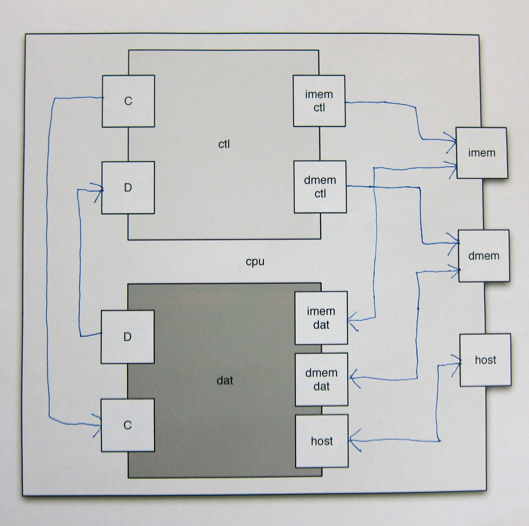
\includegraphics[width=0.9\textwidth]{../tutfigs/cpu.png} 
\end{center}

\end{columns}
\end{frame}

\begin{frame}[fragile]{CPU Interfaces}
\begin{columns}
\column{0.40\textwidth}

\begin{scala}
class RomIo extends Bundle {
  val isVal = Bool(INPUT)
  val raddr = UInt(INPUT, 32)
  val rdata = Bits(OUTPUT, 32) 
}

class RamIo extends RomIo {
  val isWr  = Bool(INPUT)
  val wdata = Bits(INPUT, 32) 
}

class CpathIo extends Bundle {
  val imem = RomIo().flip()
  val dmem = RamIo().flip()
  ... }

class DpathIo extends Bundle {
  val imem = RomIo().flip()
  val dmem = RamIo().flip()
  ... }
\end{scala}

\column{0.50\textwidth}

\begin{center}
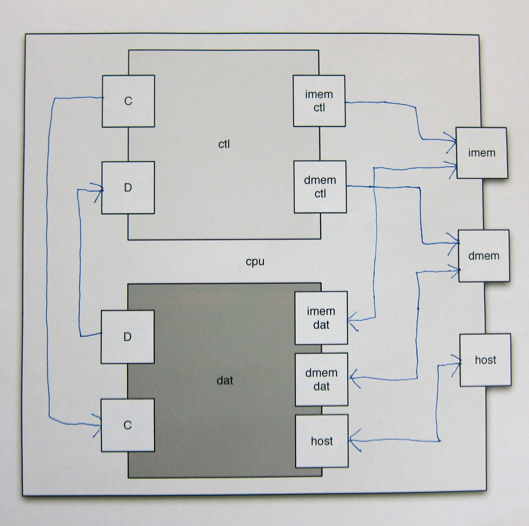
\includegraphics[width=0.9\textwidth]{../tutfigs/cpu.png} 
\end{center}

\end{columns}
\end{frame}

\begin{frame}[fragile]{Partial Interface Fulfillment}
\begin{columns}
\column{0.40\textwidth}

\begin{scala}
class Cpath extends Module {
  val io = new CpathIo();
  ...
  io.imem.isVal := ...;
  io.dmem.isVal := ...;
  io.dmem.isWr  := ...;
  ...
}

class Dpath extends Module {
  val io = new DpathIo();
  ...
  io.imem.raddr := ...;
  io.dmem.raddr := ...;
  io.dmem.wdata := ...;
  ...
}
\end{scala}

\column{0.50\textwidth}

\begin{center}
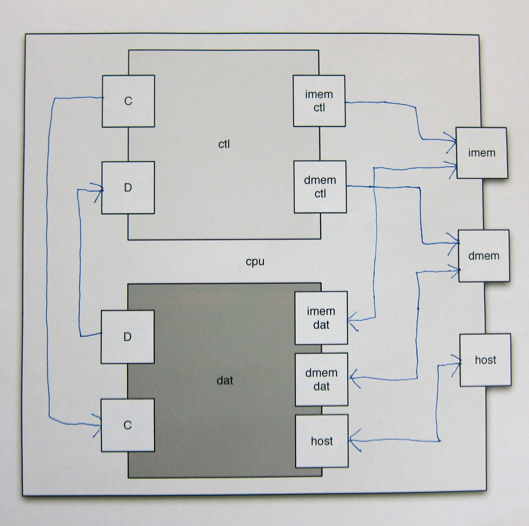
\includegraphics[width=0.9\textwidth]{../tutfigs/cpu.png} 
\end{center}

\end{columns}
\end{frame}

\begin{frame}[fragile]{Multiple Partial Bulk Connections}
\begin{columns}
\column{0.40\textwidth}

\begin{scala}
class Cpu extends Module {
  val io = new CpuIo()
  val c  = new CtlPath()
  val d  = new DatPath()
  c.io.ctl  <> d.io.ctl
  c.io.dat  <> d.io.dat
  c.io.imem <> io.imem
  d.io.imem <> io.imem
  c.io.dmem <> io.dmem
  d.io.dmem <> io.dmem
  d.io.host <> io.host
}
\end{scala}

\column{0.50\textwidth}

\begin{center}
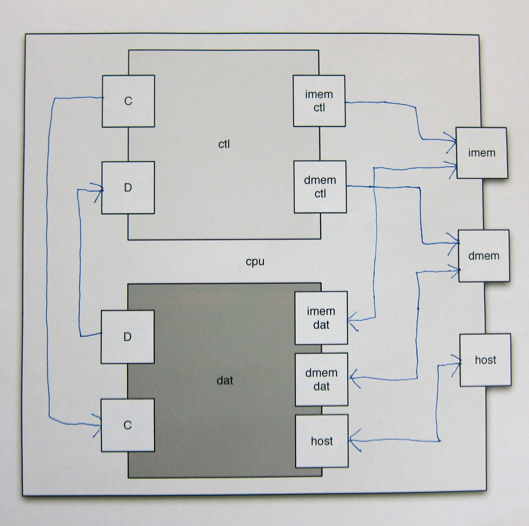
\includegraphics[width=0.9\textwidth]{../tutfigs/cpu.png} 
\end{center}

\end{columns}
\end{frame}

\begin{frame}
\begin{columns}

\column{0.65\textwidth}

\frametitle{Resources}
\begin{itemize}
\item Scala books
\item \url{chisel.eecs.berkeley.edu}
\item Chisel writings
\begin{itemize}
\item Chisel tutorial
\item Chisel manual
\item Chisel DAC-2012 paper
\end{itemize}
\item Chisel examples on github
\begin{itemize}
\item Sodor Processors
\item Floating Point Unit
\item Rocket Processor
\item Hwacha Vector Unit
\end{itemize}
\end{itemize}

\column{0.25\textwidth}

\begin{center}

\includegraphics[height=0.4\textheight]{../bootcamp/figs/programming-scala.pdf} \\
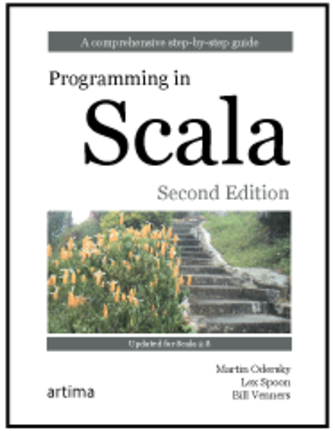
\includegraphics[height=0.4\textheight]{../bootcamp/figs/programming-in-scala.pdf}
\end{center}

\end{columns}
\end{frame}

\begin{frame}
\frametitle{Standard Library in ChiselUtil.scala}
\begin{itemize}
\item Basic Utils
\item Vecs
\item Queues
\item Arbiters
% \item Crossbars
\item Structural Memory
\end{itemize}
\end{frame}

\begin{frame}[fragile]
\frametitle{Bits Properties}
\begin{scala}
object log2Up {
  def apply(in: Int): Int = if(in == 1) 1 else ceil(log(in)/log(2)).toInt
}

object log2Down {
  def apply(x : Int): Int = if (x == 1) 1 else floor(log(x)/log(2.0)).toInt
}

object isPow2 {
  def apply(in: Int): Boolean = in > 0 && ((in & (in-1)) == 0)
}

object PopCount {
  def apply(in: Seq[Bool]): UInt = ...
  def apply(in: Bits): UInt = ...
}
\end{scala}
\end{frame}

\begin{frame}[fragile]
\frametitle{Bits Functions}
\begin{itemize}
\item LFSR16 -- random number generator
\item Reverse -- reverse order of bits
\item FillInterleaved -- space out booleans into uint
\end{itemize}
\begin{scala}
object LFSR16 {
  def apply(increment: Bool = Bool(true)): UInt = ...
}
object Reverse {
  def apply(in: UInt): UInt = ...
}
object FillInterleaved {
  def apply(n: Int, in: Bits): UInt = ...
}
\end{scala}
\end{frame}

\begin{frame}[fragile]
\frametitle{Stateful Functions}
\begin{itemize}
\item n cycle delayed version of input signal
\end{itemize}
\begin{scala}
object ShiftRegister {
  def apply[T <: Data](in: T, n: Int, en: Bool = Bool(true)): T = ...
}
\end{scala}
\begin{itemize}
\item enable driven counter with parameterized wrapping
\end{itemize}
\begin{scala}
object Counter {
  def apply(cond: Bool, n: Int): (UInt, Bool) = ...
}
\end{scala}
\end{frame}

\begin{frame}[fragile]
\frametitle{Priority Encoding Functions}
\begin{itemize}
\item UIntToOH -- returns one hot encoding of input int
\item OHToUInt -- returns int version of one hot encoding input
\item Mux1H -- builds mux tree of input vector using a one hot encoded select signal
\end{itemize}
\begin{scala}
object UIntToOH {
  def apply(in: UInt, width: Int = -1): Bits = ...
}

object OHToUInt {
  def apply(in: Seq[Bool]): UInt = ...
}

object Mux1H {
  def apply[T <: Data](sel: Vec[Bool], in: Vec[T]): T = ...
}
\end{scala}
\end{frame}

\begin{frame}[fragile]
\frametitle{Priority Mux Function}
\begin{itemize}
\item PriorityMux -- build mux tree allow multiple select signals with priority given to first select signal
\end{itemize}
\begin{scala}
object PriorityMux {
  def apply[T <: Bits](in: Seq[(Bool, T)]): T = ...
  def apply[T <: Bits](sel: Seq[Bool], in: Seq[T]): T = ...
  def apply[T <: Bits](sel: Bits, in: Seq[T]): T = ...
}
\end{scala}
\end{frame}

\begin{frame}[fragile]
\frametitle{Priority Encoding Functions}
\begin{itemize}
\item PriorityEncoder -- returns the bit position of the trailing 1 in the input vector
  with the assumption that multiple bits of the input bit vector can be set
\item PriorityEncoderOH -- returns the bit position of the trailing 1 in the input vector
  with the assumption that only one bit in the input vector can be set.
\end{itemize}
\begin{scala}
object PriorityEncoder {
  def apply(in: Seq[Bool]): UInt = ...
  def apply(in: Bits): UInt = ...
}

object PriorityEncoderOH {
  def apply(in: Bits): UInt = ...
  def apply(in: Seq[Bool]): Seq[UInt] = ...
}
\end{scala}
\end{frame}

\begin{frame}[fragile]{Vec Construction}
\begin{scala}
object Vec {
  def apply[T <: Data](elts: Seq[T]): Vec[T]
  def apply[T <: Data](elts: Vec[T]): Vec[T]
  def apply[T <: Data](elt0: T, elts: T*): Vec[T]

  def fill[T <: Data](n: Int)(f: => T): Vec[T]
  def tabulate[T <: Data](n: Int)(f: Int => T): Vec[T]
  def tabulate[T <: Data](n1: Int, n2: Int)(f: (Int, Int) => T): Vec[Vec[T]] 
}
\end{scala}
\begin{scala}
Vec(A, L, M)
Vec.fill(3){ UInt(width = 8) } ==== 
  Vec(UInt(width = 8), UInt(width = 8), UInt(width = 8))
Vec.tabulate(3){ UInt(_) } ==== 
  Vec(UInt(0), UInt(1), UInt(2))
val v = Vec.fill(0){ UInt(width = 8) }
for ...
  v += UInt(width = 8)
\end{scala}
\end{frame}


\begin{frame}[fragile]{Functional Vec}
\begin{scala}
class Vec[T <: Data](val gen: () => T) 
    extends Data with Cloneable with BufferProxy[T] { 
  ... 
  def forall(p: T => Bool): Bool
  def exists(p: T => Bool): Bool
  def contains(x: T): Bool
  def count(p: T => Bool): UInt

  def indexWhere(p: T => Bool): UInt
  def lastIndexWhere(p: T => Bool): UInt
}
\end{scala}
\begin{scala}
Vec(K, L, M).contains(x) ==== ( x === K || x === L || x === M )
\end{scala}
\end{frame}


\begin{frame}[fragile]
\frametitle{Queues}
\begin{itemize}
\item Required parameter \verb+entries+ controls depth
\item The width is determined from the inputs.
\end{itemize}
\begin{scala}
class QueueIO[T <: Data](type: T, entries: Int) extends Bundle {
  val enq   = Decoupled(data.clone).flip
  val deq   = Decoupled(data.clone)
  val count = UFix(OUTPUT, log2Up(entries+1))
}

class Queue[T <: Data]
    (type: T, entries: Int, 
     pipe: Boolean = false,
     flow: Boolean = false
     flushable: Boolean = false)
    extends Module  
\end{scala}
\begin{scala}
val q = new Queue(UInt(), 16)
q.io.enq <> producer.io.out
consumer.io.in <> q.io.deq
\end{scala}
\end{frame}

\begin{frame}[fragile]
\frametitle{Pipes}
\begin{itemize}
\item delays data coming down pipeline by \verb+latency+ cycles
\item similar to \verb+ShiftRegister+ but exposes Pipe interface
\end{itemize}
\begin{scala}
class PipeIO[+T <: Data](data: T) extends Bundle {
  val valid = Bool(OUTPUT)
  val bits  = data.clone.asOutput
}

class Pipe[T <: Data](type: T, latency: Int = 1) extends Module
\end{scala}
\begin{scala}
val pipe = new Pipe(UInt())
pipe.io.enq <> produce.io.out
consumer.io.in <> pipe.io.deq
\end{scala}
\end{frame}

\begin{frame}[fragile]
\frametitle{Fixed Priority Arbiter}
\begin{itemize}
\item sequences \verb+n+ producers into 1 consumer
\item priority is given to lower producer
\end{itemize}
\begin{scala}
class ArbiterIO[T <: Data](data: T, n: Int) extends Bundle {
  val in     = Vec.fill(n) { Decoupled(data) }.flip
  val out    = Decoupled( data.clone )
  val chosen = Bits(OUTPUT, log2Up(n))
}

class Arbiter[T <: Data](type: T, n: Int) extends Module 
\end{scala}
\begin{scala}
val arb = new Arbiter(UInt(), 2)
arb.io.in(0) <> producer0.io.out
arb.io.in(1) <> producer1.io.out
consumer.io.in <> arb.io.out
\end{scala}
\end{frame}

\begin{frame}[fragile]
\frametitle{Round Robin Arbiter}
\begin{itemize}
\item sequences \verb+n+ producers into 1 consumer
\item producers are chosen in round robin order
\end{itemize}
\begin{scala}
class ArbiterIO[T <: Data](data: T, n: Int) extends Bundle {
  val in     = Vec.fill(n) { Decoupled(data) }.flip
  val out    = Decoupled( data.clone )
  val chosen = Bits(OUTPUT, log2Up(n))
}

class RRArbiter[T <: Data](type: T, n: Int) extends Module 
\end{scala}
\begin{scala}
val arb = new RRArbiter(UInt(), 2)
arb.io.in(0) <> producer0.io.out
arb.io.in(1) <> producer1.io.out
consumer.io.in <> arb.io.out
\end{scala}
\end{frame}

% \begin{frame}[fragile]
% \frametitle{Crossbar}
% \begin{itemize}
% \item Priority
% \item Round Robin
% \end{itemize}
% \end{frame}


\begin{frame}[fragile]
\frametitle{Structural Memory}
\begin{itemize}
\item Defined number of ports
\item Port specific accesses
\end{itemize}
\begin{scala}
class FunMem[T <: Data]
    (data: T, depth: Int, numReads: Int, numWrites: Int) {
  ...
  def read(addr: UInt, idx: Int = 0): T = ...
  def write(addr: UInt, data: T, idx: Int = 0) = ...
  ...
}
\end{scala}
\begin{scala}
val cellDats = new FunMem(Bits(width = DATA_WIDTH), NUM_CELLS, 1, 1)
when (isWrite0) {
  cellDats.write(ca0, dat0, 0)
}
when (isWrite1) {
  cellDats.write(ca1, dat1, 1)
}
... cellDats.read(ca, 0) ...
... cellDats.read(ca, 1) ...
\end{scala}
\end{frame}

\begin{frame}{Acknowledgements}
\begin{itemize}
\item ``What is Chisel?'' based on slides from Patrick Li
\end{itemize}
\end{frame}

\end{document}
